% Options for packages loaded elsewhere
\PassOptionsToPackage{unicode}{hyperref}
\PassOptionsToPackage{hyphens}{url}
%
\documentclass[
  english,
  jou,floatsintext]{apa6}
\usepackage{amsmath,amssymb}
\usepackage{lmodern}
\usepackage{iftex}
\ifPDFTeX
  \usepackage[T1]{fontenc}
  \usepackage[utf8]{inputenc}
  \usepackage{textcomp} % provide euro and other symbols
\else % if luatex or xetex
  \usepackage{unicode-math}
  \defaultfontfeatures{Scale=MatchLowercase}
  \defaultfontfeatures[\rmfamily]{Ligatures=TeX,Scale=1}
\fi
% Use upquote if available, for straight quotes in verbatim environments
\IfFileExists{upquote.sty}{\usepackage{upquote}}{}
\IfFileExists{microtype.sty}{% use microtype if available
  \usepackage[]{microtype}
  \UseMicrotypeSet[protrusion]{basicmath} % disable protrusion for tt fonts
}{}
\makeatletter
\@ifundefined{KOMAClassName}{% if non-KOMA class
  \IfFileExists{parskip.sty}{%
    \usepackage{parskip}
  }{% else
    \setlength{\parindent}{0pt}
    \setlength{\parskip}{6pt plus 2pt minus 1pt}}
}{% if KOMA class
  \KOMAoptions{parskip=half}}
\makeatother
\usepackage{xcolor}
\IfFileExists{xurl.sty}{\usepackage{xurl}}{} % add URL line breaks if available
\IfFileExists{bookmark.sty}{\usepackage{bookmark}}{\usepackage{hyperref}}
\hypersetup{
  pdftitle={Study sample characteristics in chronobiology and sleep research},
  pdfauthor={Selma Tir1,2, Rhiannon White1,3, \& Manuel Spitschan1,4,5},
  pdflang={en-EN},
  pdfkeywords={demographics, ethnicity, sex, research participants, reporting, publishing, meta-science},
  hidelinks,
  pdfcreator={LaTeX via pandoc}}
\urlstyle{same} % disable monospaced font for URLs
\usepackage{graphicx}
\makeatletter
\def\maxwidth{\ifdim\Gin@nat@width>\linewidth\linewidth\else\Gin@nat@width\fi}
\def\maxheight{\ifdim\Gin@nat@height>\textheight\textheight\else\Gin@nat@height\fi}
\makeatother
% Scale images if necessary, so that they will not overflow the page
% margins by default, and it is still possible to overwrite the defaults
% using explicit options in \includegraphics[width, height, ...]{}
\setkeys{Gin}{width=\maxwidth,height=\maxheight,keepaspectratio}
% Set default figure placement to htbp
\makeatletter
\def\fps@figure{htbp}
\makeatother
\setlength{\emergencystretch}{3em} % prevent overfull lines
\providecommand{\tightlist}{%
  \setlength{\itemsep}{0pt}\setlength{\parskip}{0pt}}
\setcounter{secnumdepth}{-\maxdimen} % remove section numbering
% Make \paragraph and \subparagraph free-standing
\ifx\paragraph\undefined\else
  \let\oldparagraph\paragraph
  \renewcommand{\paragraph}[1]{\oldparagraph{#1}\mbox{}}
\fi
\ifx\subparagraph\undefined\else
  \let\oldsubparagraph\subparagraph
  \renewcommand{\subparagraph}[1]{\oldsubparagraph{#1}\mbox{}}
\fi
% Manuscript styling
\usepackage{upgreek}
\captionsetup{font=singlespacing,justification=justified}

% Table formatting
\usepackage{longtable}
\usepackage{lscape}
% \usepackage[counterclockwise]{rotating}   % Landscape page setup for large tables
\usepackage{multirow}		% Table styling
\usepackage{tabularx}		% Control Column width
\usepackage[flushleft]{threeparttable}	% Allows for three part tables with a specified notes section
\usepackage{threeparttablex}            % Lets threeparttable work with longtable

% Create new environments so endfloat can handle them
% \newenvironment{ltable}
%   {\begin{landscape}\begin{center}\begin{threeparttable}}
%   {\end{threeparttable}\end{center}\end{landscape}}
\newenvironment{lltable}{\begin{landscape}\begin{center}\begin{ThreePartTable}}{\end{ThreePartTable}\end{center}\end{landscape}}

% Enables adjusting longtable caption width to table width
% Solution found at http://golatex.de/longtable-mit-caption-so-breit-wie-die-tabelle-t15767.html
\makeatletter
\newcommand\LastLTentrywidth{1em}
\newlength\longtablewidth
\setlength{\longtablewidth}{1in}
\newcommand{\getlongtablewidth}{\begingroup \ifcsname LT@\roman{LT@tables}\endcsname \global\longtablewidth=0pt \renewcommand{\LT@entry}[2]{\global\advance\longtablewidth by ##2\relax\gdef\LastLTentrywidth{##2}}\@nameuse{LT@\roman{LT@tables}} \fi \endgroup}

% \setlength{\parindent}{0.5in}
% \setlength{\parskip}{0pt plus 0pt minus 0pt}

% \usepackage{etoolbox}
\makeatletter
\patchcmd{\HyOrg@maketitle}
  {\section{\normalfont\normalsize\abstractname}}
  {\section*{\normalfont\normalsize\abstractname}}
  {}{\typeout{Failed to patch abstract.}}
\patchcmd{\HyOrg@maketitle}
  {\section{\protect\normalfont{\@title}}}
  {\section*{\protect\normalfont{\@title}}}
  {}{\typeout{Failed to patch title.}}
\makeatother
\shorttitle{Study sample characteristics in chronobiology and sleep research}
\keywords{demographics, ethnicity, sex, research participants, reporting, publishing, meta-science\newline\indent Word count: X}
\usepackage{dblfloatfix}


\usepackage{lineno}

\linenumbers
\usepackage{csquotes}
\usepackage[titles]{tocloft}
\cftpagenumbersoff{figure}
\renewcommand{\cftfigpresnum}{\itshape\figurename\enspace}
\renewcommand{\cftfigaftersnum}{.\space}
\setlength{\cftfigindent}{0pt}
\setlength{\cftafterloftitleskip}{0pt}
\settowidth{\cftfignumwidth}{Figure 10.\qquad}
\ifXeTeX
  % Load polyglossia as late as possible: uses bidi with RTL langages (e.g. Hebrew, Arabic)
  \usepackage{polyglossia}
  \setmainlanguage[]{english}
\else
  \usepackage[main=english]{babel}
% get rid of language-specific shorthands (see #6817):
\let\LanguageShortHands\languageshorthands
\def\languageshorthands#1{}
\fi
\ifLuaTeX
  \usepackage{selnolig}  % disable illegal ligatures
\fi
\newlength{\cslhangindent}
\setlength{\cslhangindent}{1.5em}
\newlength{\csllabelwidth}
\setlength{\csllabelwidth}{3em}
\newenvironment{CSLReferences}[2] % #1 hanging-ident, #2 entry spacing
 {% don't indent paragraphs
  \setlength{\parindent}{0pt}
  % turn on hanging indent if param 1 is 1
  \ifodd #1 \everypar{\setlength{\hangindent}{\cslhangindent}}\ignorespaces\fi
  % set entry spacing
  \ifnum #2 > 0
  \setlength{\parskip}{#2\baselineskip}
  \fi
 }%
 {}
\usepackage{calc}
\newcommand{\CSLBlock}[1]{#1\hfill\break}
\newcommand{\CSLLeftMargin}[1]{\parbox[t]{\csllabelwidth}{#1}}
\newcommand{\CSLRightInline}[1]{\parbox[t]{\linewidth - \csllabelwidth}{#1}\break}
\newcommand{\CSLIndent}[1]{\hspace{\cslhangindent}#1}

\title{Study sample characteristics in chronobiology and sleep research}
\author{Selma Tir\textsuperscript{1,2}, Rhiannon White\textsuperscript{1,3}, \& Manuel Spitschan\textsuperscript{1,4,5}}
\date{}


\authornote{

Corresponding author: Manuel Spitschan (\href{mailto:manuel.spitschan@psy.ox.ac.uk}{\nolinkurl{manuel.spitschan@psy.ox.ac.uk}}). This work ws funded by the Wellcome Trust (Sir Henry Wellcome Fellowship to MS 204686/Z/16/Z; Research Enrichment -- Diversity \& Inclusion WT 204686/Z/16/A) and Linacre College (Biomedical Sciences Junior Research Fellowship to MS).

The authors made the following contributions. Selma Tir: Data curation, Investigation, Software, Visualization, Writing -- original draft, Writing -- review \& editing; Rhiannon White: Investigation, Writing -- original draft, Writing -- review \& editing; Manuel Spitschan: Conceptualization, Data curation, Funding acquisition, Investigation, Methodology, Project administration, Software, Writing -- original draft, Writing -- review \& editing.

}

\affiliation{\vspace{0.5cm}\textsuperscript{1} Department of Experimental Psychology, University of Oxford\\\textsuperscript{2} Sleep and Circadian Neuroscience Institute, Nuffield Department of Clinical Neurosciences, University of Oxford\\\textsuperscript{3} Warwick Medical School, University of Warwick, United Kingdom\\\textsuperscript{4} Centre for Chronobiology, Psychiatric Hospital of the University of Basel, Switzerland\\\textsuperscript{5} Transfaculty Research Platform Molecular and Cognitive Neurosciences, University of Basel, Switzerland}

\abstract{
Many aspects of sleep and circadian physiology appear to be sensitive to participant-level characteristics. While recent research robustly highlights the importance of considering participant-level demographic information, it is not clear to what extent this information is available in the large body of already published literature. Here, we investigated study sample characteristics in the published sleep and chronobiology research over the past 40 years. 6,777 articles were identified and a random sample of 20\% was included. The reporting of sample size, age, sex, gender, ethnicity, level of education, socio-economic status, and profession of the study population was scored, and any reported aggregate summary statistics for these variables were recorded. We found that while \textgreater90\% of studies reported age or sex, all other variables were reported in \textless10\% of cases. Sex balance greatly changed over the years, from a \textasciitilde3:1 male to female ratio in the 1990s to a near-equal representation in the 2010s. We found that the majority of studies report at least sex or age, while other variables are typically not reported. Reporting quality is highly variable, indicating an opportunity to standardize reporting guidelines for participant-level characteristics to facilitate meta analyses.
}



\begin{document}
\maketitle

\hypertarget{introduction}{%
\section{Introduction}\label{introduction}}

Many aspects of sleep and circadian physiology appear to be sensitive to characteristics of the studied population, most notably sex (Anderson \& FitzGerald, 2020; Cain et al., 2010; Mong et al., 2011; Redline et al., 2004; Santhi et al., 2016), age (Benloucif et al., 2006; Bliwise, 1993; Desforges, Prinz, Vitiello, Raskind, \& Thorpy, 1990; Duffy, Zitting, \& Chinoy, 2015; Espiritu, 2008; Li, Vitiello, \& Gooneratne, 2018; Mander, Winer, \& Walker, 2017; Redline et al., 2004) and ethnicity (Ahn et al., 2021; Eastman, Molina, Dziepak, \& Smith, 2012; Eastman, Tomaka, \& Crowley, 2016; Goldstein, Gaston, McGrath, \& Jackson, 2020). More generally, there is a large literature on individual differences on sleep and circadian physiology (Baehr, Revelle, \& Eastman, 2000; Burgess \& Fogg, 2008; Chellappa, 2021; Dongen, Vitellaro, \& Dinges, 2005; Horne \& Östberg, 1977; Kerkhof, 1985; Santhi et al., 2012; Tankova, Adan, \& Buela-Casal, 1994), demonstrating the need to consider participant-level data.

The extent to which a scientific field's findings are generalisable depend very much on the representativeness of a given study sample. As an example, a recent study reviewed the reporting and analysis of sex in biological sciences research (Woitowich, Beery, \& Woodruff, 2020). The authors found that while sex inclusion has significantly increased over the past 10 years (Beery \& Zucker, 2011), sex-based analysis has not improved, despite recent policies and funder mandates (Clayton \& Collins, 2014).

While research findings converge on participant-level demographic characteristics affecting outcomes, it is not clear to what extent this information is available in the large body of already published literature, nor to what extent it is even reported. Here, we address the question of participant-level demographic characteristics (age, sex, gender, ethnicity, level of education, socio-economic status, and profession of the study population) and reporting thereof in chronobiology and sleep research. Here, we extracted the study sample characteristics in a total of 1356 randomly sampled publications across the 8 top (ranked by the Journal Impact Factor) chronobiology and sleep research and subjected them to a comprehensive analysis.

\hypertarget{methods}{%
\section{Methods}\label{methods}}

\emph{Procedure}. Journal articles published between 1979 and 2019 (odd years) in the top eight sleep and chronobiology journals were considered. The listing of possible of target journals was based on a previously established list of journals implementing a hybrid strategy by consulting the Web of Science Master Journal List, domain-relevant expertise in sleep and chronobiology and consulting with a senior researcher with \textgreater25 years of experience in the field (Spitschan, Schmidt, \& Blume, 2020). From this previously derived list, we selected eight journals were selected based on their five-year Impact Factor, and included \emph{Journal of Pineal Research} (ISSN: 0742-3098 / 1600-079X; 2018 5-year IF: 12.197), \emph{Sleep} (0161-8105 / 1550-9109; 5.588), \emph{Journal of Sleep Research} (0962-1105 / 1365-2869; 3.951), \emph{Sleep Medicine} (1389-9457 / 1878-5506; 3.934), \emph{Journal of Clinical Sleep Medicine} (1550-9389 / 1550-9397; 3.855), \emph{Journal of Biological Rhythms} (0748-7304 / 1552-4531; 3.349), Behavioral Sleep Medicine (1540-2002 / 1540-2010; 3.162), and \emph{Chronobiology International} (0742-0528 / 1525-6073; 2.998). While \emph{Sleep Medicine Reviews} also features in the list of journals, we did not include it as it primarily publishes reviews.

\emph{Article inclusion}. 6,777 articles were identified through a MEDLINE search by the journal and including odd years. A random sample of 20\% was initially selected for screening. Inclusion requirements included conducting original research in the English language, reporting human data, and recruiting volunteers. As such, animal studies, bibliographies, case reports, comments, conference proceedings, editorials, guidelines, letters, retracted publications, reviews, errata and corrigenda were excluded.

\emph{Review and article extraction}. All included articles were reviewed for eligibility and coded by RW. The reporting of sample size, age, sex, gender, ethnicity, level of education, socioeconomic status, and profession of the study population was scored binarily (0 = not reported, 1 = reported), and any reported aggregate summary statistics for these variables were recorded. Funding source, geographical location and clinical focus of the article were examined, as well as whether data were analyzed by including any of the demographic variables as covariates.

Data were coded in an Excel Spreadsheet and analyzed in R Studio (version 4.0.5). Reporting of funding, geographical location, and number of sub-studies for each article were investigated for the sample of articles that passed all eligibility criteria.

\emph{Pre-registration}. We pre-registered our protocol (specified using the PRISMA-P template (PRISMA-P Group et al., 2015; Shamseer et al., 2015)) on the Open Science Framework (\url{https://osf.io/cu3we/}).

\emph{Materials, data and code availability}. All data underlying this manuscript are available on a public GitHub repository (\url{https://github.com/hcvnl/sleep_circadian_demographics_data}). The article was written in R (R Core Team, 2021) using RMarkdown and papaja (Aust \& Barth, 2020), employing a series of additional R packages (Arnold, 2021; Attali \& Baker, 2019; Auguie, 2017; Bates \& Maechler, 2021; Borchers, 2021; Edwards, 2020; Henry, Wickham, \& Chang, 2020; Kaplan \& Pruim, 2021; Morey \& Rouder, 2018; Müller \& Wickham, 2021; Pruim, Kaplan, \& Horton, 2021; Pruim, Kaplan, \& Horton, 2017; Sarkar, 2008; Sarkar \& Andrews, 2019; Wei \& Simko, 2017; Wickham, 2007, 2016, 2019, 2021; Wickham \& Bryan, 2019; Wickham, François, Henry, \& Müller, 2021; Wickham \& Hester, 2020; Wilke, 2021; Xiao, 2018; Xie, 2015) and is fully reproducible.

\hypertarget{results}{%
\section{Results}\label{results}}

\hypertarget{inclusion-exclusion}{%
\subsubsection{Inclusion \& Exclusion}\label{inclusion-exclusion}}

85\% of the sampled articles met eligibility criteria during the review.

\begin{figure}
\centering
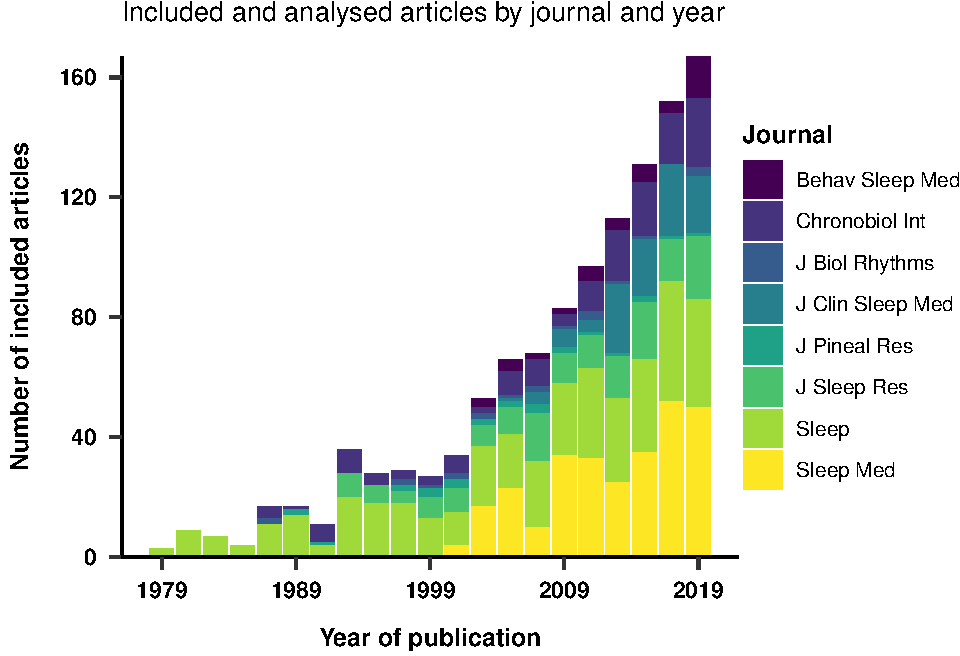
\includegraphics{article_files/figure-latex/unnamed-chunk-1-1.pdf}
\caption{\label{fig:unnamed-chunk-1}Funding sources and geographical location of the studies. A. Reporting of funding across the years. B. Distribution of articles by study location. The eight most represented countries are individually shown.}
\end{figure}

\begin{figure}
\centering
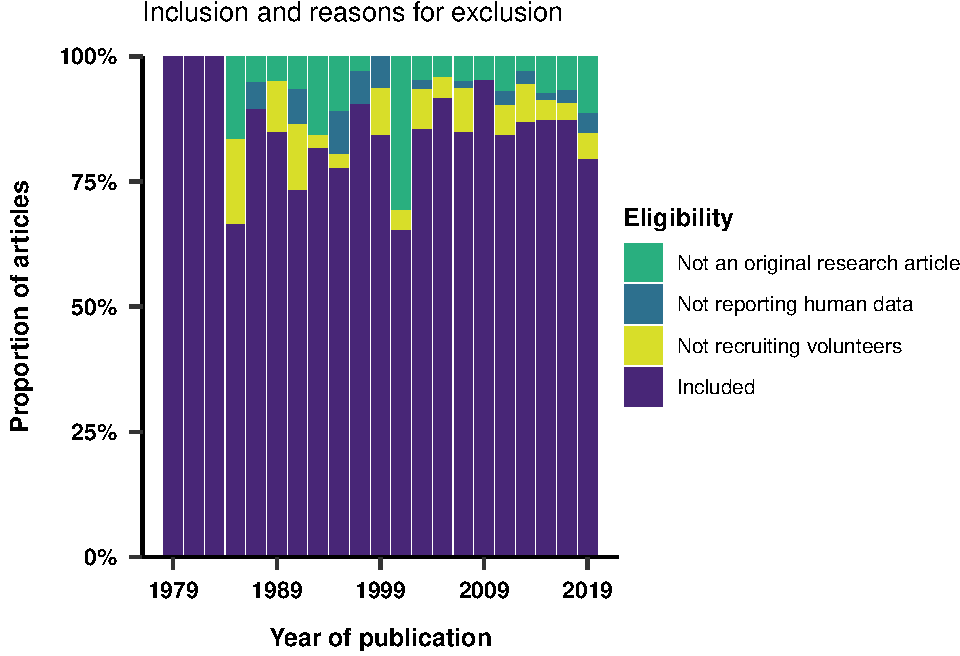
\includegraphics{article_files/figure-latex/unnamed-chunk-2-1.pdf}
\caption{\label{fig:unnamed-chunk-2}Funding sources and geographical location of the studies. A. Reporting of funding across the years. B. Distribution of articles by study location. The eight most represented countries are individually shown.}
\end{figure}

\hypertarget{funding}{%
\subsubsection{Funding}\label{funding}}

Funding sources were reported by 62\% of studies, while funding number was also reported in 69\% of these cases. Overall, funding by the United States' National Institutes of Health (NIH) represented 19\% of the reported funding agencies. 92\% of the studies funded by the NIH also reported funding number. The second most represented funding agencies were the Australian National Health and Medical Research Council (NHMRC) and the Canadian Institutes of Health Research (CIHR).

\begin{figure}
\centering
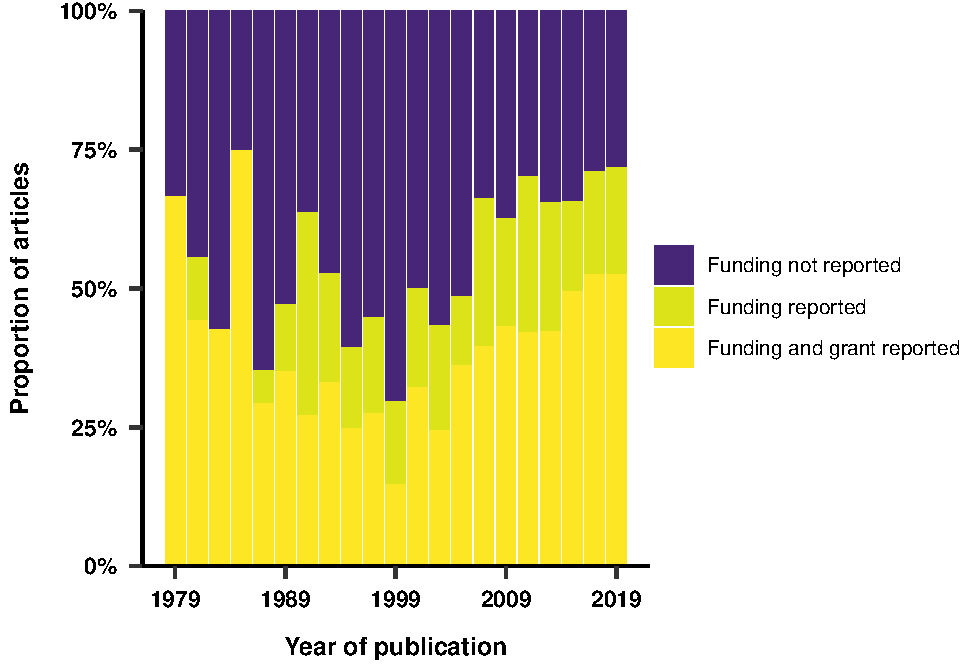
\includegraphics{article_files/figure-latex/unnamed-chunk-3-1.pdf}
\caption{\label{fig:unnamed-chunk-3}Funding sources and geographical location of the studies. A. Reporting of funding across the years. B. Distribution of articles by study location. The eight most represented countries are individually shown.}
\end{figure}

\hypertarget{geographical-location}{%
\subsubsection{Geographical location}\label{geographical-location}}

93\% of articles were conducted in a single country. The geographical location of the study was explicitly reported in 57\% of studies. The country of study was inferred for the rest of the sampled articles. Inference was primarily based on the first author's affiliation. Overall, 53 countries were represented. 77\% of articles reported multiple countries of study. Figure 2B shows the distribution of study location across time with the eight most represented countries.

\begin{figure}
\centering
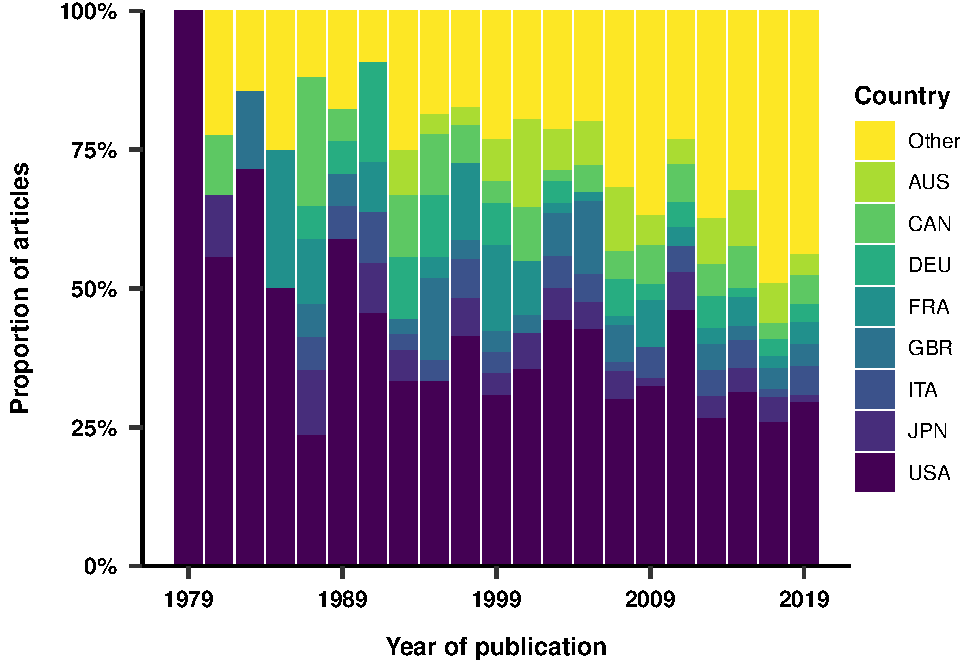
\includegraphics{article_files/figure-latex/unnamed-chunk-4-1.pdf}
\caption{\label{fig:unnamed-chunk-4}Funding sources and geographical location of the studies. A. Reporting of funding across the years. B. Distribution of articles by study location. The eight most represented countries are individually shown.}
\end{figure}

\hypertarget{sample-size}{%
\subsubsection{Sample size}\label{sample-size}}

Sample size was reported in 92\% of studies, while 98\% investigated a single sampled population.

\begin{figure}
\centering
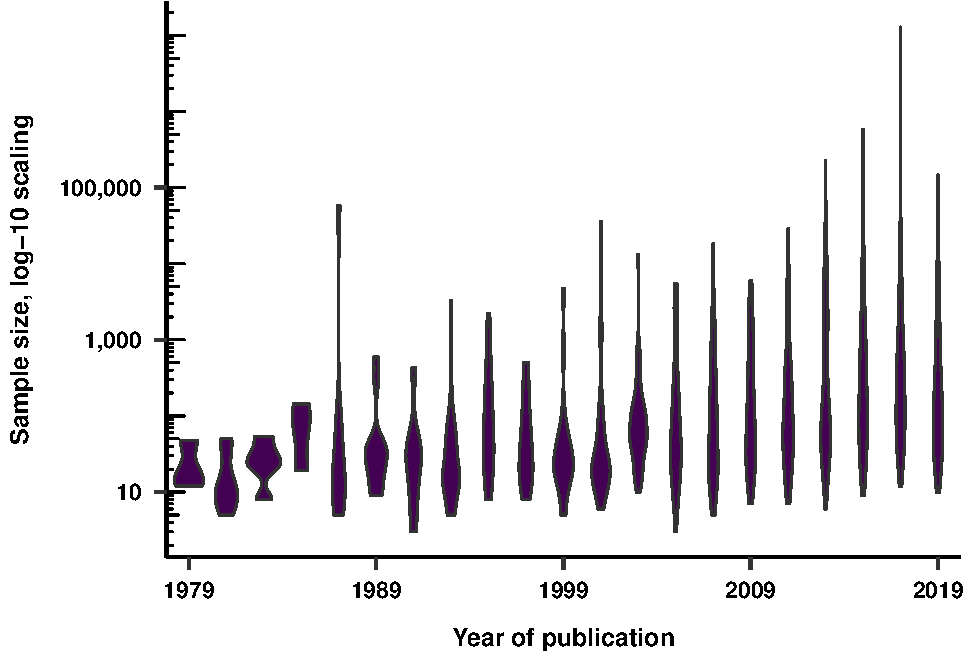
\includegraphics{article_files/figure-latex/unnamed-chunk-5-1.pdf}
\caption{\label{fig:unnamed-chunk-5}Sample size of the recruited volunteers. Numbers are computed with a log-10 scale.}
\end{figure}

\hypertarget{age}{%
\subsubsection{Age}\label{age}}

93\% of articles reported a variable describing age. Figure 4A and 4B show the use of various age variables by year and journal of publication. Overall, the mean age of the study populations was 39 years old.

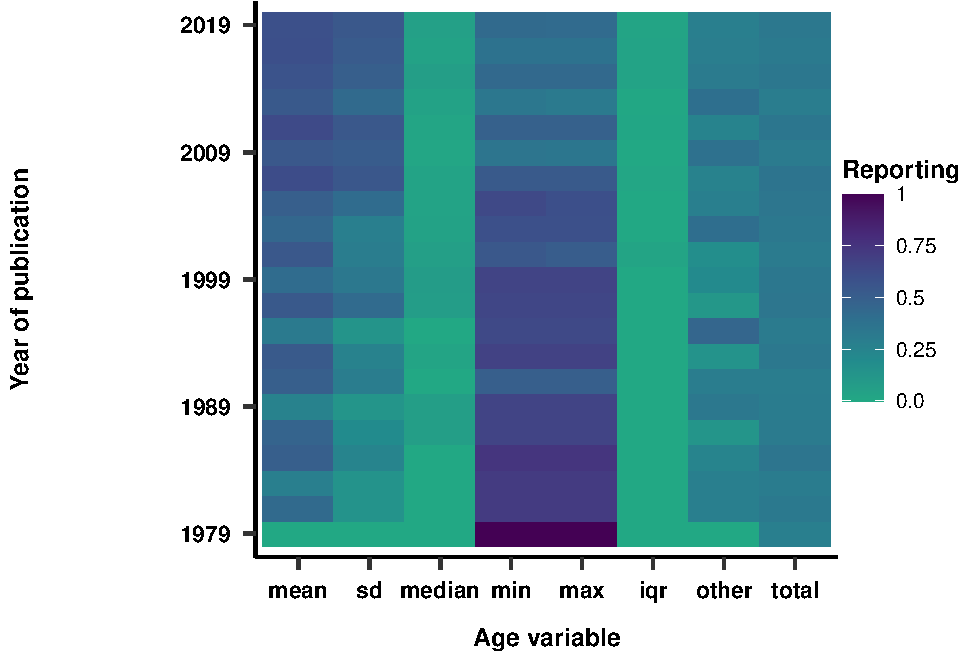
\includegraphics{article_files/figure-latex/unnamed-chunk-6-1.pdf}
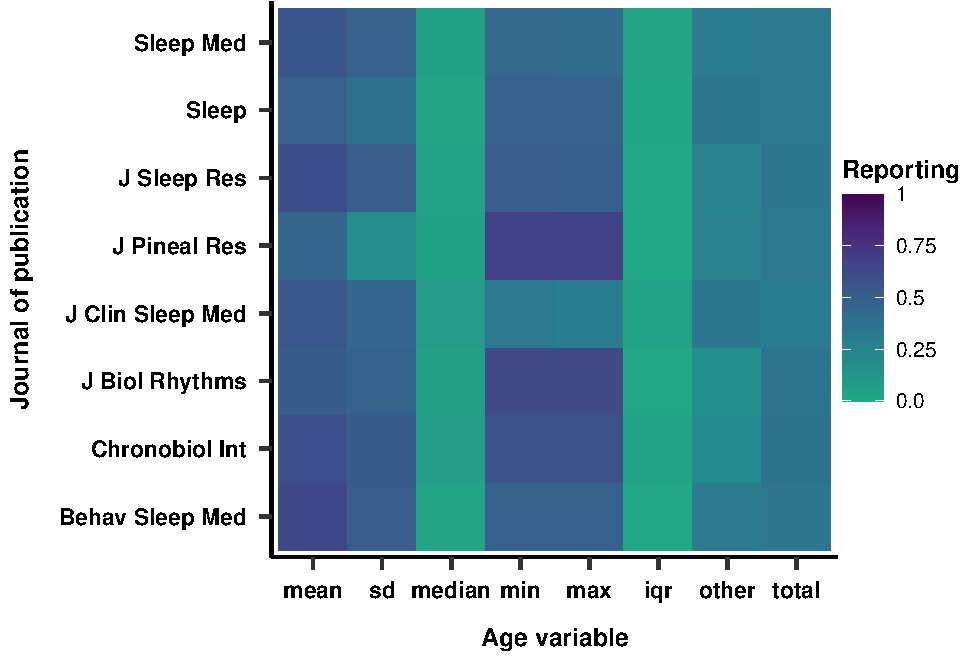
\includegraphics{article_files/figure-latex/unnamed-chunk-7-1.pdf}

\begin{figure}
\centering
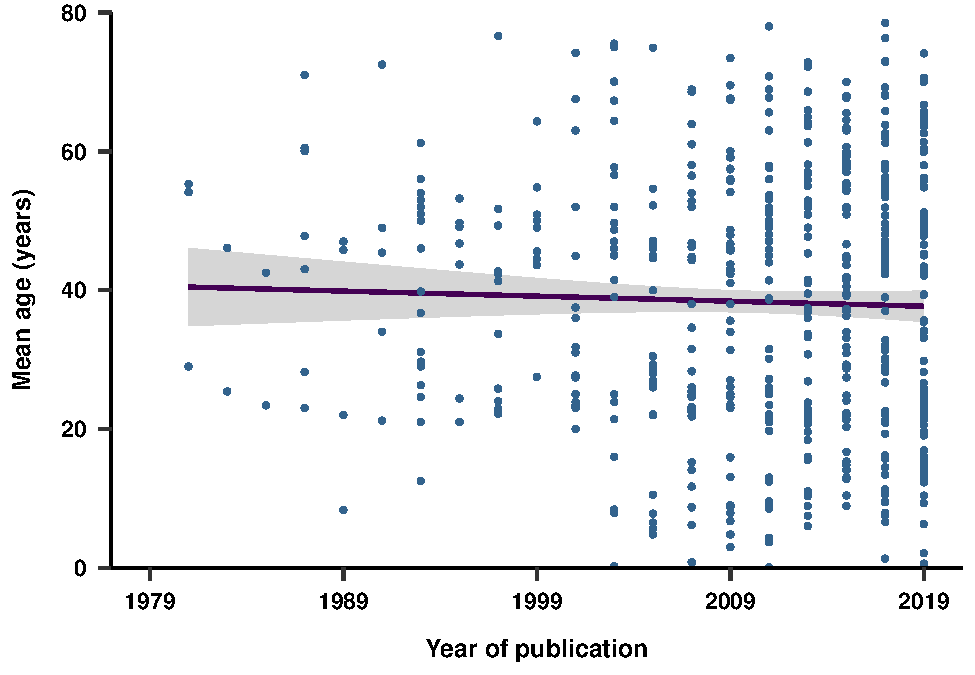
\includegraphics{article_files/figure-latex/unnamed-chunk-8-1.pdf}
\caption{\label{fig:unnamed-chunk-8}Reporting of age variables. Correlation between the reporting of the mean, standrad deviation of the mean, median, minimum, maximum, interquartile range and other age variables by A. year of publication and B. journal of publication. C. Mean age by year of publication.}
\end{figure}

\hypertarget{sex}{%
\subsubsection{Sex}\label{sex}}

Sex was reported in 89\% of the studies. Figure 5 displays the proportion of studies that recruited male subjects, female subjects, both sexes or did not specify the sex of the participants. 13\% of the studies reporting sex only recruited male participants, while 10\% only employed females. Out of the studies focusing on a single gender, 1\% of the male studies focused on a sex dependent feature, while 2\% of the female studies did. 4\% of studies reported age by sex.

\begin{figure}
\centering
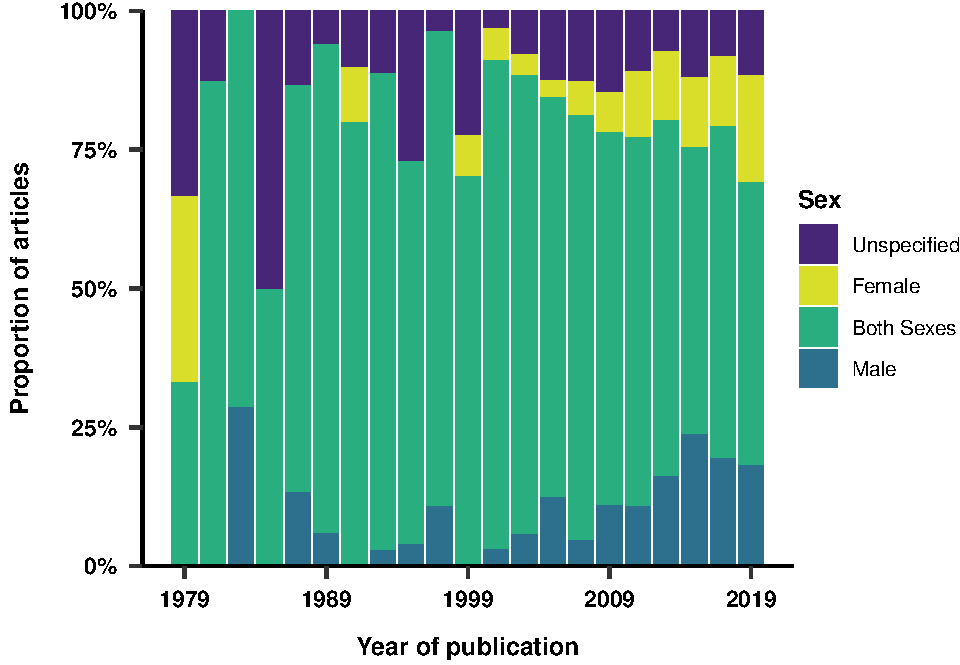
\includegraphics{article_files/figure-latex/unnamed-chunk-9-1.pdf}
\caption{\label{fig:unnamed-chunk-9}Sex inclusion. Proportion of studies that recruited male subjects, female subjects, both sexes, or did not specify the sex of the participants.}
\end{figure}

\hypertarget{ethnicity-education-profession-and-socio-economic-status}{%
\subsubsection{Ethnicity, education, profession and socio-economic status}\label{ethnicity-education-profession-and-socio-economic-status}}

Other demographics variables were reported in 12\% of studies for education, 15\% for ethnicity, 2\% for profession, and 4\% for socio-economic status. Figure 6 shows the distribution of this reporting across the years. Figures 7 show the number of categories reported for each variable.

\begin{figure}
\centering
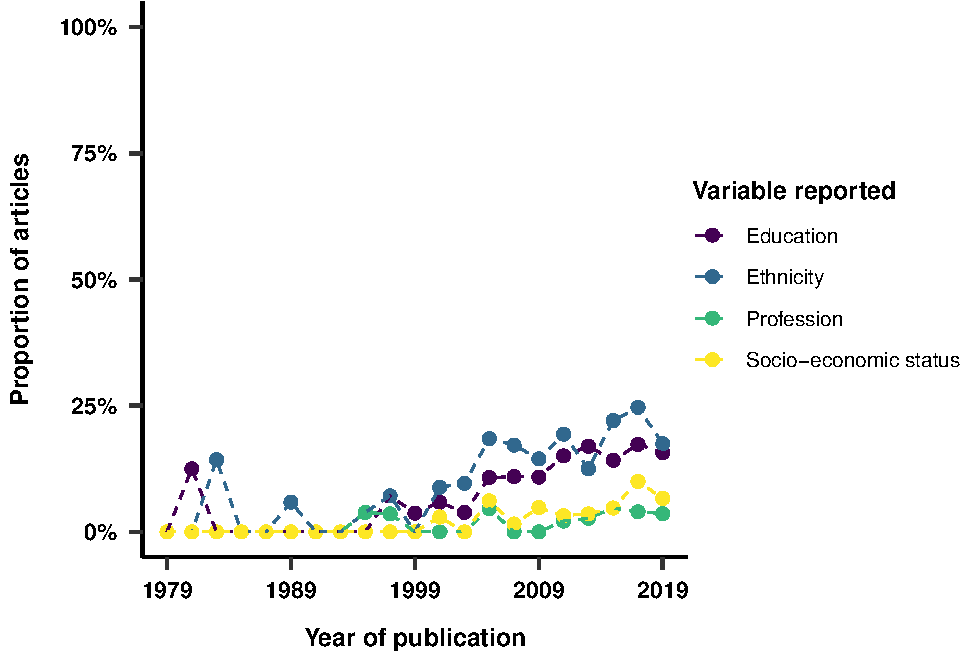
\includegraphics{article_files/figure-latex/unnamed-chunk-10-1.pdf}
\caption{\label{fig:unnamed-chunk-10}Reporting of education, ethinicity, profession and socio-economic status.}
\end{figure}

\begin{figure}
\centering
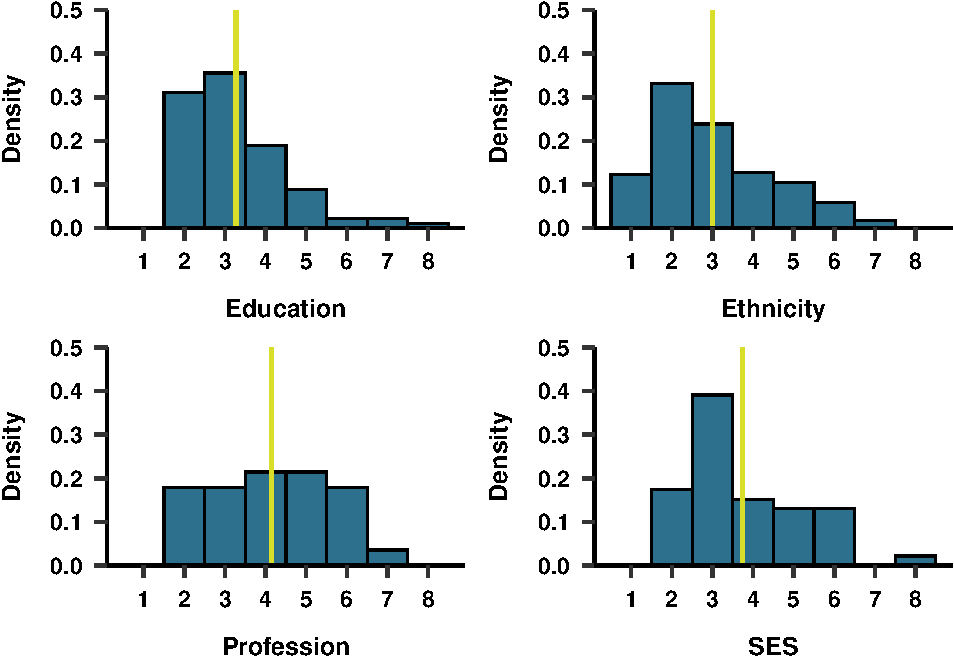
\includegraphics{article_files/figure-latex/unnamed-chunk-11-1.pdf}
\caption{\label{fig:unnamed-chunk-11}Number of categories reported for education, ethnicity, profession and socio-economic status.}
\end{figure}

\hypertarget{study-focus}{%
\subsubsection{Study focus}\label{study-focus}}

3\% of articles focused on a sex dependent feature, while 50\% investigated a clinical feature. 1\% of studies focused on twins, 1\% on pregnant women, 2\% on shift workers and 4\% on university students.

\hypertarget{analysis-disaggregation}{%
\subsubsection{Analysis disaggregation}\label{analysis-disaggregation}}

A

\begin{figure}
\centering
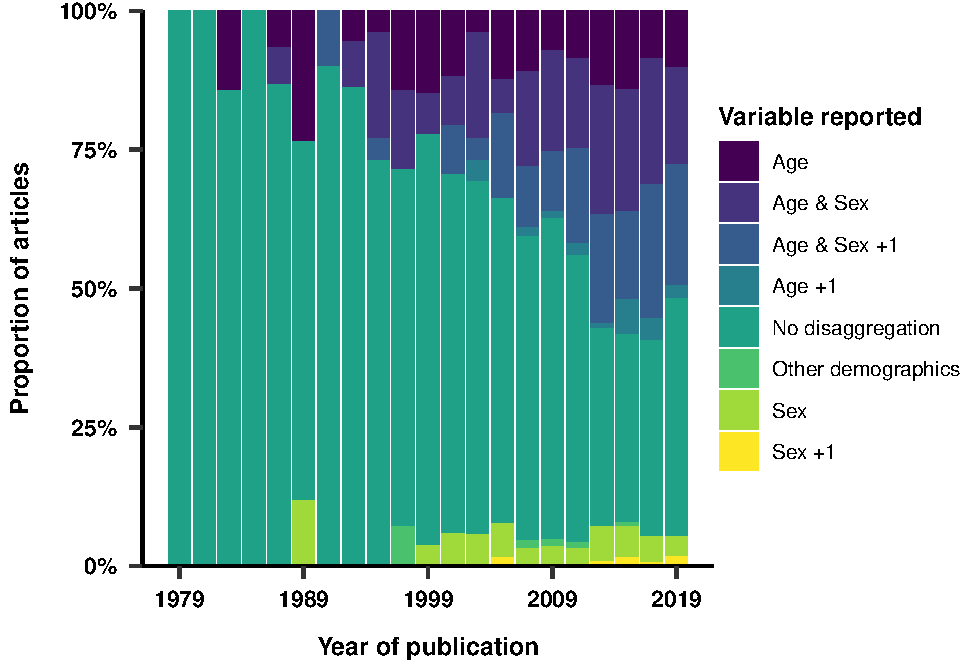
\includegraphics{article_files/figure-latex/unnamed-chunk-12-1.pdf}
\caption{\label{fig:unnamed-chunk-12}Use of study population characteristics as variables in the analysis.}
\end{figure}

\hypertarget{discussion}{%
\section{Discussion}\label{discussion}}

In the clinical domain, the need to time therapy based on a patient's individual circadian rhythm has more recently become the focus of the emerging field of chronotherapy or chronotherapeutics (Adam, 2019; Dijk \& Duffy, 2020; Greco \& Sassone-Corsi, 2020; Hill, Innominato, Lévi, \& Ballesta, 2020).

The ability to generalise findings from the scientific literature to wide and diverse populations of people hinges upon the representativeness of the study sample with respect to demographic categories. The question to what extent the composition of a given study sample can make the generalisability of findings difficult or impossible has received attention in the field of psychology, where many articles published in prominent journals reflected participants from WEIRD (Western, Educated, Industrialized, Rich, and Democratic) contexts (Henrich, Heine, \& Norenzayan, 2010; Muthukrishna et al., 2020).

\hypertarget{conclusion}{%
\section{Conclusion}\label{conclusion}}

\newpage

\hypertarget{references}{%
\section{References}\label{references}}

\begingroup
\setlength{\parindent}{-0.5in}
\setlength{\leftskip}{0.5in}

\hypertarget{refs}{}
\begin{CSLReferences}{1}{0}
\leavevmode\vadjust pre{\hypertarget{ref-adam_core_2019}{}}%
Adam, D. (2019). Core {Concept}: {Emerging} science of chronotherapy offers big opportunities to optimize drug delivery. \emph{Proceedings of the National Academy of Sciences}, \emph{116}(44), 21957--21959. \url{https://doi.org/10.1073/pnas.1916118116}

\leavevmode\vadjust pre{\hypertarget{ref-ahn_scoping_2021}{}}%
Ahn, S., Lobo, J. M., Logan, J. G., Kang, H., Kwon, Y., \& Sohn, M.-W. (2021). A scoping review of racial/ethnic disparities in sleep. \emph{Sleep Medicine}, \emph{81}, 169--179. \url{https://doi.org/10.1016/j.sleep.2021.02.027}

\leavevmode\vadjust pre{\hypertarget{ref-anderson_sexual_2020}{}}%
Anderson, S. T., \& FitzGerald, G. A. (2020). Sexual dimorphism in body clocks. \emph{Science (New York, N.Y.)}, \emph{369}(6508), 1164--1165. \url{https://doi.org/10.1126/science.abd4964}

\leavevmode\vadjust pre{\hypertarget{ref-R-ggthemes}{}}%
Arnold, J. B. (2021). \emph{Ggthemes: Extra themes, scales and geoms for 'ggplot2'}. Retrieved from \url{https://CRAN.R-project.org/package=ggthemes}

\leavevmode\vadjust pre{\hypertarget{ref-R-ggExtra}{}}%
Attali, D., \& Baker, C. (2019). \emph{ggExtra: Add marginal histograms to 'ggplot2', and more 'ggplot2' enhancements}. Retrieved from \url{https://CRAN.R-project.org/package=ggExtra}

\leavevmode\vadjust pre{\hypertarget{ref-R-gridExtra}{}}%
Auguie, B. (2017). \emph{gridExtra: Miscellaneous functions for "grid" graphics}. Retrieved from \url{https://CRAN.R-project.org/package=gridExtra}

\leavevmode\vadjust pre{\hypertarget{ref-R-papaja}{}}%
Aust, F., \& Barth, M. (2020). \emph{{papaja}: {Create} {APA} manuscripts with {R Markdown}}. Retrieved from \url{https://github.com/crsh/papaja}

\leavevmode\vadjust pre{\hypertarget{ref-baehr_individual_2000}{}}%
Baehr, E. K., Revelle, W., \& Eastman, C. I. (2000). Individual differences in the phase and amplitude of the human circadian temperature rhythm: With an emphasis on morningness-eveningness: {Phase} and amplitude of the temperature rhythm. \emph{Journal of Sleep Research}, \emph{9}(2), 117--127. \url{https://doi.org/10.1046/j.1365-2869.2000.00196.x}

\leavevmode\vadjust pre{\hypertarget{ref-R-Matrix}{}}%
Bates, D., \& Maechler, M. (2021). \emph{Matrix: Sparse and dense matrix classes and methods}. Retrieved from \url{https://CRAN.R-project.org/package=Matrix}

\leavevmode\vadjust pre{\hypertarget{ref-beery_sex_2011}{}}%
Beery, A. K., \& Zucker, I. (2011). Sex bias in neuroscience and biomedical research. \emph{Neuroscience and Biobehavioral Reviews}, \emph{35}(3), 565--572. \url{https://doi.org/10.1016/j.neubiorev.2010.07.002}

\leavevmode\vadjust pre{\hypertarget{ref-benloucif_responsiveness_2006}{}}%
Benloucif, S., Green, K., L'Hermite-Balériaux, M., Weintraub, S., Wolfe, L. F., \& Zee, P. C. (2006). Responsiveness of the aging circadian clock to light. \emph{Neurobiology of Aging}, \emph{27}(12), 1870--1879. \url{https://doi.org/10.1016/j.neurobiolaging.2005.10.011}

\leavevmode\vadjust pre{\hypertarget{ref-bliwise_sleep_1993}{}}%
Bliwise, D. L. (1993). Sleep in {Normal} {Aging} and {Dementia}. \emph{Sleep}, \emph{16}(1), 40--81. \url{https://doi.org/10.1093/sleep/16.1.40}

\leavevmode\vadjust pre{\hypertarget{ref-R-pracma}{}}%
Borchers, H. W. (2021). \emph{Pracma: Practical numerical math functions}. Retrieved from \url{https://CRAN.R-project.org/package=pracma}

\leavevmode\vadjust pre{\hypertarget{ref-burgess_individual_2008}{}}%
Burgess, H. J., \& Fogg, L. F. (2008). Individual {Differences} in the {Amount} and {Timing} of {Salivary} {Melatonin} {Secretion}. \emph{PLoS ONE}, \emph{3}(8), e3055. \url{https://doi.org/10.1371/journal.pone.0003055}

\leavevmode\vadjust pre{\hypertarget{ref-cain_sex_2010}{}}%
Cain, S. W., Dennison, C. F., Zeitzer, J. M., Guzik, A. M., Khalsa, S. B. S., Santhi, N., \ldots{} Duffy, J. F. (2010). Sex differences in phase angle of entrainment and melatonin amplitude in humans. \emph{Journal of Biological Rhythms}, \emph{25}(4), 288--296. \url{https://doi.org/10.1177/0748730410374943}

\leavevmode\vadjust pre{\hypertarget{ref-chellappa_individual_2021}{}}%
Chellappa, S. L. (2021). Individual differences in light sensitivity affect sleep and circadian rhythms. \emph{Sleep}, \emph{44}(2), zsaa214. \url{https://doi.org/10.1093/sleep/zsaa214}

\leavevmode\vadjust pre{\hypertarget{ref-clayton_policy_2014}{}}%
Clayton, J. A., \& Collins, F. S. (2014). Policy: {NIH} to balance sex in cell and animal studies. \emph{Nature}, \emph{509}(7500), 282--283. \url{https://doi.org/10.1038/509282a}

\leavevmode\vadjust pre{\hypertarget{ref-desforges_sleep_1990}{}}%
Desforges, J. F., Prinz, P. N., Vitiello, M. V., Raskind, M. A., \& Thorpy, M. J. (1990). Sleep {Disorders} and {Aging}. \emph{New England Journal of Medicine}, \emph{323}(8), 520--526. \url{https://doi.org/10.1056/NEJM199008233230805}

\leavevmode\vadjust pre{\hypertarget{ref-dijk_novel_2020}{}}%
Dijk, D.-J., \& Duffy, J. F. (2020). Novel {Approaches} for {Assessing} {Circadian} {Rhythmicity} in {Humans}: {A} {Review}. \emph{Journal of Biological Rhythms}, \emph{35}(5), 421--438. \url{https://doi.org/10.1177/0748730420940483}

\leavevmode\vadjust pre{\hypertarget{ref-van_dongen_individual_2005}{}}%
Dongen, H. P. A. van, Vitellaro, K. M., \& Dinges, D. F. (2005). Individual {Differences} in {Adult} {Human} {Sleep} and {Wakefulness}: {Leitmotif} for a {Research} {Agenda}. \emph{Sleep}, \emph{28}(4), 479--498. \url{https://doi.org/10.1093/sleep/28.4.479}

\leavevmode\vadjust pre{\hypertarget{ref-duffy_aging_2015}{}}%
Duffy, J. F., Zitting, K.-M., \& Chinoy, E. D. (2015). Aging and {Circadian} {Rhythms}. \emph{Sleep Medicine Clinics}, \emph{10}(4), 423--434. \url{https://doi.org/10.1016/j.jsmc.2015.08.002}

\leavevmode\vadjust pre{\hypertarget{ref-eastman_blacks_2012}{}}%
Eastman, C. I., Molina, T. A., Dziepak, M. E., \& Smith, M. R. (2012). Blacks ({African} {Americans}) have shorter free-running circadian periods than whites ({Caucasian} {Americans}). \emph{Chronobiology International}, \emph{29}(8), 1072--1077. \url{https://doi.org/10.3109/07420528.2012.700670}

\leavevmode\vadjust pre{\hypertarget{ref-eastman_circadian_2016}{}}%
Eastman, C. I., Tomaka, V. A., \& Crowley, S. J. (2016). Circadian rhythms of {European} and {African}-{Americans} after a large delay of sleep as in jet lag and night work. \emph{Scientific Reports}, \emph{6}(1), 36716. \url{https://doi.org/10.1038/srep36716}

\leavevmode\vadjust pre{\hypertarget{ref-R-lemon}{}}%
Edwards, S. M. (2020). \emph{Lemon: Freshing up your 'ggplot2' plots}. Retrieved from \url{https://CRAN.R-project.org/package=lemon}

\leavevmode\vadjust pre{\hypertarget{ref-espiritu_aging-related_2008}{}}%
Espiritu, J. R. D. (2008). Aging-{Related} {Sleep} {Changes}. \emph{Clinics in Geriatric Medicine}, \emph{24}(1), 1--14. \url{https://doi.org/10.1016/j.cger.2007.08.007}

\leavevmode\vadjust pre{\hypertarget{ref-goldstein_sleep_2020}{}}%
Goldstein, S. J., Gaston, S. A., McGrath, J. A., \& Jackson, C. L. (2020). Sleep {Health} and {Serious} {Psychological} {Distress}: {A} {Nationally} {Representative} {Study} of the {United} {States} among {White}, {Black}, and {Hispanic}/{Latinx} {Adults}. \emph{Nature and Science of Sleep}, \emph{12}, 1091--1104. \url{https://doi.org/10.2147/NSS.S268087}

\leavevmode\vadjust pre{\hypertarget{ref-greco_personalized_2020}{}}%
Greco, C. M., \& Sassone-Corsi, P. (2020). Personalized medicine and circadian rhythms: {Opportunities} for modern society. \emph{Journal of Experimental Medicine}, \emph{217}(6), e20200702. \url{https://doi.org/10.1084/jem.20200702}

\leavevmode\vadjust pre{\hypertarget{ref-henrich_weirdest_2010}{}}%
Henrich, J., Heine, S. J., \& Norenzayan, A. (2010). The weirdest people in the world? \emph{Behavioral and Brain Sciences}, \emph{33}(2-3), 61--83. \url{https://doi.org/10.1017/S0140525X0999152X}

\leavevmode\vadjust pre{\hypertarget{ref-R-ggstance}{}}%
Henry, L., Wickham, H., \& Chang, W. (2020). \emph{Ggstance: Horizontal 'ggplot2' components}. Retrieved from \url{https://CRAN.R-project.org/package=ggstance}

\leavevmode\vadjust pre{\hypertarget{ref-hill_optimizing_2020}{}}%
Hill, R. J. W., Innominato, P. F., Lévi, F., \& Ballesta, A. (2020). Optimizing circadian drug infusion schedules towards personalized cancer chronotherapy. \emph{PLOS Computational Biology}, \emph{16}(1), e1007218. \url{https://doi.org/10.1371/journal.pcbi.1007218}

\leavevmode\vadjust pre{\hypertarget{ref-horne_individual_1977}{}}%
Horne, J. A., \& Östberg, O. (1977). Individual differences in human circadian rhythms. \emph{Biological Psychology}, \emph{5}(3), 179--190. \url{https://doi.org/10.1016/0301-0511(77)90001-1}

\leavevmode\vadjust pre{\hypertarget{ref-R-ggformula}{}}%
Kaplan, D., \& Pruim, R. (2021). \emph{Ggformula: Formula interface to the grammar of graphics}. Retrieved from \url{https://CRAN.R-project.org/package=ggformula}

\leavevmode\vadjust pre{\hypertarget{ref-kerkhof_inter-individual_1985}{}}%
Kerkhof, G. A. (1985). Inter-individual differences in the human circadian system: {A} review. \emph{Biological Psychology}, \emph{20}(2), 83--112. \url{https://doi.org/10.1016/0301-0511(85)90019-5}

\leavevmode\vadjust pre{\hypertarget{ref-li_sleep_2018}{}}%
Li, J., Vitiello, M. V., \& Gooneratne, N. S. (2018). Sleep in {Normal} {Aging}. \emph{Sleep Medicine Clinics}, \emph{13}(1), 1--11. \url{https://doi.org/10.1016/j.jsmc.2017.09.001}

\leavevmode\vadjust pre{\hypertarget{ref-mander_sleep_2017}{}}%
Mander, B. A., Winer, J. R., \& Walker, M. P. (2017). Sleep and {Human} {Aging}. \emph{Neuron}, \emph{94}(1), 19--36. \url{https://doi.org/10.1016/j.neuron.2017.02.004}

\leavevmode\vadjust pre{\hypertarget{ref-mong_sleep_2011}{}}%
Mong, J. A., Baker, F. C., Mahoney, M. M., Paul, K. N., Schwartz, M. D., Semba, K., \& Silver, R. (2011). Sleep, rhythms, and the endocrine brain: Influence of sex and gonadal hormones. \emph{The Journal of Neuroscience: The Official Journal of the Society for Neuroscience}, \emph{31}(45), 16107--16116. \url{https://doi.org/10.1523/JNEUROSCI.4175-11.2011}

\leavevmode\vadjust pre{\hypertarget{ref-R-BayesFactor}{}}%
Morey, R. D., \& Rouder, J. N. (2018). \emph{BayesFactor: Computation of bayes factors for common designs}. Retrieved from \url{https://CRAN.R-project.org/package=BayesFactor}

\leavevmode\vadjust pre{\hypertarget{ref-muthukrishna_beyond_2020}{}}%
Muthukrishna, M., Bell, A. V., Henrich, J., Curtin, C. M., Gedranovich, A., McInerney, J., \& Thue, B. (2020). Beyond {Western}, {Educated}, {Industrial}, {Rich}, and {Democratic} ({WEIRD}) {Psychology}: {Measuring} and {Mapping} {Scales} of {Cultural} and {Psychological} {Distance}. \emph{Psychological Science}, \emph{31}(6), 678--701. \url{https://doi.org/10.1177/0956797620916782}

\leavevmode\vadjust pre{\hypertarget{ref-R-tibble}{}}%
Müller, K., \& Wickham, H. (2021). \emph{Tibble: Simple data frames}. Retrieved from \url{https://CRAN.R-project.org/package=tibble}

\leavevmode\vadjust pre{\hypertarget{ref-prisma-p_group_preferred_2015}{}}%
PRISMA-P Group, Moher, D., Shamseer, L., Clarke, M., Ghersi, D., Liberati, A., \ldots{} Stewart, L. A. (2015). Preferred reporting items for systematic review and meta-analysis protocols ({PRISMA}-{P}) 2015 statement. \emph{Systematic Reviews}, \emph{4}(1), 1. \url{https://doi.org/10.1186/2046-4053-4-1}

\leavevmode\vadjust pre{\hypertarget{ref-R-mosaicData}{}}%
Pruim, R., Kaplan, D., \& Horton, N. (2021). \emph{mosaicData: Project MOSAIC data sets}. Retrieved from \url{https://CRAN.R-project.org/package=mosaicData}

\leavevmode\vadjust pre{\hypertarget{ref-R-mosaic}{}}%
Pruim, R., Kaplan, D. T., \& Horton, N. J. (2017). The mosaic package: Helping students to 'think with data' using r. \emph{The R Journal}, \emph{9}(1), 77--102. Retrieved from \url{https://journal.r-project.org/archive/2017/RJ-2017-024/index.html}

\leavevmode\vadjust pre{\hypertarget{ref-R-base}{}}%
R Core Team. (2021). \emph{R: A language and environment for statistical computing}. Vienna, Austria: R Foundation for Statistical Computing. Retrieved from \url{https://www.R-project.org/}

\leavevmode\vadjust pre{\hypertarget{ref-redline_effects_2004}{}}%
Redline, S., Kirchner, H. L., Quan, S. F., Gottlieb, D. J., Kapur, V., \& Newman, A. (2004). The effects of age, sex, ethnicity, and sleep-disordered breathing on sleep architecture. \emph{Archives of Internal Medicine}, \emph{164}(4), 406--418. \url{https://doi.org/10.1001/archinte.164.4.406}

\leavevmode\vadjust pre{\hypertarget{ref-santhi_sex_2016}{}}%
Santhi, N., Lazar, A. S., McCabe, P. J., Lo, J. C., Groeger, J. A., \& Dijk, D.-J. (2016). Sex differences in the circadian regulation of sleep and waking cognition in humans. \emph{Proceedings of the National Academy of Sciences of the United States of America}, \emph{113}(19), E2730--2739. \url{https://doi.org/10.1073/pnas.1521637113}

\leavevmode\vadjust pre{\hypertarget{ref-santhi_spectral_2012}{}}%
Santhi, N., Thorne, H. C., Veen, D. R. van der, Johnsen, S., Mills, S. L., Hommes, V., \ldots{} Dijk, D.-J. (2012). The spectral composition of evening light and individual differences in the suppression of melatonin and delay of sleep in humans: {Artificial} evening light suppresses melatonin and delays sleep. \emph{Journal of Pineal Research}, \emph{53}(1), 47--59. \url{https://doi.org/10.1111/j.1600-079X.2011.00970.x}

\leavevmode\vadjust pre{\hypertarget{ref-R-lattice}{}}%
Sarkar, D. (2008). \emph{Lattice: Multivariate data visualization with r}. New York: Springer. Retrieved from \url{http://lmdvr.r-forge.r-project.org}

\leavevmode\vadjust pre{\hypertarget{ref-R-latticeExtra}{}}%
Sarkar, D., \& Andrews, F. (2019). \emph{latticeExtra: Extra graphical utilities based on lattice}. Retrieved from \url{https://CRAN.R-project.org/package=latticeExtra}

\leavevmode\vadjust pre{\hypertarget{ref-shamseer_preferred_2015}{}}%
Shamseer, L., Moher, D., Clarke, M., Ghersi, D., Liberati, A., Petticrew, M., \ldots{} the PRISMA-P Group. (2015). Preferred reporting items for systematic review and meta-analysis protocols ({PRISMA}-{P}) 2015: Elaboration and explanation. \emph{BMJ}, \emph{349}(jan02 1), g7647--g7647. \url{https://doi.org/10.1136/bmj.g7647}

\leavevmode\vadjust pre{\hypertarget{ref-spitschan_transparency_2020}{}}%
Spitschan, M., Schmidt, M. H., \& Blume, C. (2020). Transparency and open science principles in reporting guidelines in sleep research and chronobiology journals. \emph{Wellcome Open Research}, \emph{5}, 172. \url{https://doi.org/10.12688/wellcomeopenres.16111.1}

\leavevmode\vadjust pre{\hypertarget{ref-tankova_circadian_1994}{}}%
Tankova, I., Adan, A., \& Buela-Casal, G. (1994). Circadian typology and individual differences. {A} review. \emph{Personality and Individual Differences}, \emph{16}(5), 671--684. \url{https://doi.org/10.1016/0191-8869(94)90209-7}

\leavevmode\vadjust pre{\hypertarget{ref-R-corrplot2017}{}}%
Wei, T., \& Simko, V. (2017). \emph{R package "corrplot": Visualization of a correlation matrix}. Retrieved from \url{https://github.com/taiyun/corrplot}

\leavevmode\vadjust pre{\hypertarget{ref-R-reshape2}{}}%
Wickham, H. (2007). Reshaping data with the {reshape} package. \emph{Journal of Statistical Software}, \emph{21}(12), 1--20. Retrieved from \url{http://www.jstatsoft.org/v21/i12/}

\leavevmode\vadjust pre{\hypertarget{ref-R-ggplot2}{}}%
Wickham, H. (2016). \emph{ggplot2: Elegant graphics for data analysis}. Springer-Verlag New York. Retrieved from \url{https://ggplot2.tidyverse.org}

\leavevmode\vadjust pre{\hypertarget{ref-R-stringr}{}}%
Wickham, H. (2019). \emph{Stringr: Simple, consistent wrappers for common string operations}. Retrieved from \url{https://CRAN.R-project.org/package=stringr}

\leavevmode\vadjust pre{\hypertarget{ref-R-tidyr}{}}%
Wickham, H. (2021). \emph{Tidyr: Tidy messy data}. Retrieved from \url{https://CRAN.R-project.org/package=tidyr}

\leavevmode\vadjust pre{\hypertarget{ref-R-readxl}{}}%
Wickham, H., \& Bryan, J. (2019). \emph{Readxl: Read excel files}. Retrieved from \url{https://CRAN.R-project.org/package=readxl}

\leavevmode\vadjust pre{\hypertarget{ref-R-dplyr}{}}%
Wickham, H., François, R., Henry, L., \& Müller, K. (2021). \emph{Dplyr: A grammar of data manipulation}. Retrieved from \url{https://CRAN.R-project.org/package=dplyr}

\leavevmode\vadjust pre{\hypertarget{ref-R-readr}{}}%
Wickham, H., \& Hester, J. (2020). \emph{Readr: Read rectangular text data}. Retrieved from \url{https://CRAN.R-project.org/package=readr}

\leavevmode\vadjust pre{\hypertarget{ref-R-ggridges}{}}%
Wilke, C. O. (2021). \emph{Ggridges: Ridgeline plots in 'ggplot2'}. Retrieved from \url{https://CRAN.R-project.org/package=ggridges}

\leavevmode\vadjust pre{\hypertarget{ref-woitowich_10-year_2020}{}}%
Woitowich, N. C., Beery, A., \& Woodruff, T. (2020). A 10-year follow-up study of sex inclusion in the biological sciences. \emph{eLife}, \emph{9}, e56344. \url{https://doi.org/10.7554/eLife.56344}

\leavevmode\vadjust pre{\hypertarget{ref-R-ggsci}{}}%
Xiao, N. (2018). \emph{Ggsci: Scientific journal and sci-fi themed color palettes for 'ggplot2'}. Retrieved from \url{https://CRAN.R-project.org/package=ggsci}

\leavevmode\vadjust pre{\hypertarget{ref-R-knitr}{}}%
Xie, Y. (2015). \emph{Dynamic documents with {R} and knitr} (2nd ed.). Boca Raton, Florida: Chapman; Hall/CRC. Retrieved from \url{https://yihui.org/knitr/}

\end{CSLReferences}

\endgroup


\clearpage
\renewcommand{\listfigurename}{Figure captions}


\end{document}
